\documentclass[12pt]{article}

\usepackage{graphics}
\usepackage{amsmath}
\usepackage{amsfonts}
\usepackage{amssymb}
\usepackage[table]{xcolor}



%\usepackage[active]{srcltx} % SRC Specials for DVI Searching

% Over-full v-boxes on even pages are due to the \v{c} in author's name
\vfuzz2pt % Don't report over-full v-boxes if over-edge is small

% THEOREM Environments ---------------------------------------------------

 \newtheorem{thm}{Theorem}[section]
 \newtheorem{cor}[thm]{Corollary}
 \newtheorem{lem}[thm]{Lemma}
 \newtheorem{prop}[thm]{Proposition}
 %\theoremstyle{definition}
 \newtheorem{defn}[thm]{Definition}
 %\theoremstyle{remark}
 \newtheorem{rem}[thm]{Remark}
 \numberwithin{equation}{section}
% MATH -------------------------------------------------------------------
 \DeclareMathOperator{\RE}{Re}
 \DeclareMathOperator{\IM}{Im}
 \DeclareMathOperator{\ess}{ess}
 \newcommand{\eps}{\varepsilon}
 \newcommand{\To}{\longrightarrow}
 \newcommand{\h}{\mathcal{H}}
 \newcommand{\s}{\mathcal{S}}
 \newcommand{\A}{\mathcal{A}}
 \newcommand{\J}{\mathcal{J}}
 \newcommand{\M}{\mathcal{M}}
 \newcommand{\W}{\mathcal{W}}
 \newcommand{\X}{\mathcal{X}}
 \newcommand{\BOP}{\mathbf{B}}
 \newcommand{\BH}{\mathbf{B}(\mathcal{H})}
 \newcommand{\KH}{\mathcal{K}(\mathcal{H})}
 \newcommand{\Real}{\mathbb{R}}
 \newcommand{\Complex}{\mathbb{C}}
 \newcommand{\Field}{\mathbb{F}}
 \newcommand{\RPlus}{\Real^{+}}
 \newcommand{\Polar}{\mathcal{P}_{\s}}
 \newcommand{\Poly}{\mathcal{P}(E)}
 \newcommand{\EssD}{\mathcal{D}}
 \newcommand{\Lom}{\mathcal{L}}
 \newcommand{\States}{\mathcal{T}}
 \newcommand{\abs}[1]{\left\vert#1\right\vert}
 \newcommand{\set}[1]{\left\{#1\right\}}
 \newcommand{\seq}[1]{\left<#1\right>}
 \newcommand{\norm}[1]{\left\Vert#1\right\Vert}
 \newcommand{\essnorm}[1]{\norm{#1}_{\ess}}
\usepackage{graphicx}
\usepackage{amsmath}
\usepackage{amsfonts}
\usepackage{amssymb}
%TCIDATA{OutputFilter=latex2.dll}
%TCIDATA{CSTFile=LaTeX article (bright).cst}
%TCIDATA{Created=Fri Nov 02 10:44:42 2001}
%TCIDATA{LastRevised=Mon Dec 10 11:56:49 2001}
%TCIDATA{<META NAME="GraphicsSave" CONTENT="32">}
%TCIDATA{<META NAME="DocumentShell" CONTENT="General\Blank Document">}
%TCIDATA{Language=American English}
\newtheorem{theorem}{Theorem}
\newtheorem{acknowledgment}[theorem]{Acknowledgment}
\newtheorem{algorithm}[theorem]{Algorithm}
\newtheorem{axiom}[theorem]{Axiom}
\newtheorem{case}[theorem]{Case}
\newtheorem{claim}[theorem]{Claim}
\newtheorem{conclusion}[theorem]{Conclusion}
\newtheorem{condition}[theorem]{Condition}
\newtheorem{conjecture}[theorem]{Conjecture}
\newtheorem{corollary}[theorem]{Corollary}
\newtheorem{criterion}[theorem]{Criterion}
\newtheorem{definition}[theorem]{Definition}
\newtheorem{example}[theorem]{Example}
\newtheorem{exercise}[theorem]{Exercise}
\newtheorem{lemma}[theorem]{Lemma}
\newtheorem{notation}[theorem]{Notation}
\newtheorem{problem}[theorem]{Problem}
\newtheorem{proposition}[theorem]{Proposition}
\newtheorem{remark}[theorem]{Remark}
\newtheorem{solution}[theorem]{Solution}
\newtheorem{summary}[theorem]{Summary}
\newenvironment{proof}[1][Proof]{\textbf{#1.} }{\ \rule{0.5em}{0.5em}}
\renewcommand\refname{}
\renewcommand\thefootnote{}
\textheight=9in \topmargin=-0.6in \everymath{\displaystyle}
\textwidth=6.5in \oddsidemargin=0.05in
\renewcommand\arraystretch{1.5}
\newenvironment{amatrix}[1]{%
  \left[\begin{array}{@{}*{#1}{c}|c@{}}
}{%
  \end{array}\right]
}
\includeonly{}
\usepackage{amsfonts}
\usepackage{amssymb}
\usepackage{eucal}
\usepackage{multicol}
\usepackage[bw]{mcode}
\usepackage{listings}
\everymath{\displaystyle}
\graphicspath{{C:/Users/michael/Documents/Graduate School/Stochastic Processes and Modeling/}}

\begin{document}

{\large\bf MATH 6600, Homework 1, 10-2-2015}

\vspace{6 ex}

{\bf Name: Michael Hennessey} \hfill

\vspace{6 ex}

\begin{enumerate}
\item The Dreams of the Nineties are Alive...
      \begin{enumerate}
      \item You'd like to plan the least amount of time to spend in town so that when you return to the camera repair shop, there is at least a probability $p$ that the repair on your camera is complete.  After how long should you return to check on your camera?\\

Since we are counting the number of events happening in a time period, (Bernoulli trials with small probability of success) we follow Poisson law. Additionally, as the number of events happening in two disjoint intervals of time are independent, we know that the number of cameras repaired over time can be modelled as a Poisson process. Therefore, the probability density function for  m cameras repaired in time t is 
$$P_m(t)=\frac{a^mt^m}{m!}e^{-at}.$$
Thus for each $t$, $X_t$, where $X_t$ is the random variable denoting the number of cameras repaired at time $t$, follows a Poisson distribution with parameter $at$. In particular, the mean number of repairs in time $t$ is $at$. Therefore, if we look at the mean number of repairs in 1 hour, we have $a=\frac{1}{\tau}$. From what Fred and Carrie said, there are $k+1$ cameras that must be repaired before Aimee begins working on mine. Thus to determine the best time to come back, we focus on the probability corresponding to $m=k+2$. Then we have
$$\frac{1}{2}<p=\int_0^\lambda P_{k+2}(t)dt=\int_0^\lambda\frac{t^{k+2}}{\tau^{k+2}(k+2)!}e^{-t/\tau}dt$$
Notice that this is equal to $\tau $ times the gamma cumulative distribution function with scale $\tau $ and shape $k+3$. Therefore, the appropriate time to return to check on my camera will be the time $\lambda$ that satisfies the equation above, which can be better expressed as
$$p=\tau\int_0^\lambda\frac{t^{k+2}}{\tau^{k+3}(k+2)!}e^{-t/\tau}dt=\tau GammaCDF(t,k+3,\tau).$$

\item Suppose the average camera repair time is one hour, choose a reasonable value for $p$, and evaluate your optimal waiting time for $k=0,...,5$. Comment on your answers.

If the average camera repair time is one, we have $\tau=1$. I will choose $p=.85$ to calculate the optimal waiting times. We will use the formula devloped in the previous part of the question and the Table A.4 (The Incomplete Gamma Function) in the book Modern Mathematical Statistics with Applications  by Devore and Berk to determine the numerical answers.
\begin{itemize}
\item For $k=0$ we have
$$p=.85=GammaCDF(t,3,1)$$
Then, using the table, we linearly interpolate between the two points
$$GammaCDF(5,3,1)=.875 \text{ and } GammaCDF(4,3,1)=.762$$
Then we see that the appropriate return time for the chosen probability is $t=4.78$ hours. We follow the same process for the next five calculations.
\item For $k=1$ the appropriate return time is $t=6.01$ hours.
\item For $k=2$ the appropriate return time is $t=7.32$ hours.
\item For $k=3$ the appropriate return time is $t=8.55$ hours.
\item For $k=4$ the appropriate return time is $t=9.74$ hours.
\item For $k=5$ the appropriate return time is $t=10.91$ hours.
\end{itemize}

\item Good day: Aimee is working on a camera but  $k=0$ cameras are waiting. Your non-technical companion smacks you and says, obviously if the average camera repair time is one hour, and Aimee is in the middle of repair on a camera, you should simply return in 90 minutes. If you follow this strategy, what is the probability that the repair on your camera will be done when you return? What is the probabilty that Aimee hasn't even started working on your camera when you return? How long would you have waited before returning according to your optimal strategy worked out above? How much better is your strategy than your companion's simply reasoned strategy?\\

 If I return in 90 minutes, the probability that my camera will be done is $$GammaCDF(1.5,3,1)=.202$$ (found by linearly interpolating $GammaCDF(1,3,1)$ and $GammaCDF(2,3,1)$.) The probability that Aimee has not started working on the camera is the same as the complement of the probability that Aimee has finished the first camera. It is computed thus
$$p=1-GammaCDF(1.5,2,1)=1-.429=.571.$$
If we had waited until we had a $.85$ probability for camera repair completion, we would have not come back until 4.78 hours after we dropped the camera off. We can see that my strategy is better in the sense that a 10-fold increase in probability of camera repair results from a 3.19-fold increase in time waited. We also note that the probability Aimee hasn't started working on my camera after 4.78 hours have passed is a meager .0514. Then even if Aimee hadn't finished my camera, she would almost certainly be working on it. To illustrate, we examime two strategies: first, we stay in the shop until the camera is completed after we wait the first 90 minutes. Second, if we were to come back each 90 minutes to check on the camera, there would only be a .577 probability of completion at the second check. The third check at 4.5 hours would finally have a probability of completion of about .8. Thus, my friend's strategy would either require us to remain in the shop for multiple hours to wait for the camera's completion or remain close enough to the shop to check back every 90 minutes, whereas my strategy would allow us to explore Portlandia for almost 5 hours. We might not get any pictures, but at least we would spend our time doing something fun.

\item Bad day: Aimee is working on a camera and a large number $k$ of cameras are also waiting to be repaired. For your particular $p$ value, describe the behavior of the ratio of your planned time to return to the expected time for completion of repair on your camera as the number $k$ of cameras waiting to be repaired becomes large. Describe more generally how this ratio behaves for a general fixed value of $p$ as $k$ becomes large. Interpret and connect to any mathematical principles of which you may be aware. \\

As evidenced by the calculated values above,for a fixed value $p$, the amount of additional waiting time for a new camera added to the the queue is a little more than one. If we were to calculate times for larger values of $k$, we would see that the added waiting time per camera approaches $\tau=1$. Therefore, as $k$ approaches infinity, the added waiting time will be extremely close to the average repair time. Then, as the added waiting time per camera approaches the average repair time, the sample mean $\bar{X}_n=\frac{X_1+...+X_{k+2}}{k+2}$ will approach the average repair time. This is the phenomena called the Law of Large Numbers. In fact, this is the strong case and we have 
$$Pr\{\lim_{k\to\infty}\bar{X}_{k+2}=\tau\}=1.$$
Therefore, the ratio of planned time to return to the expected time for completion of repair on my camera as $k$ number of cameras waiting to be repaired becomes large approaches 1.


\end{enumerate}

\item Leaving the Line\\

Suppose that the incoming service requests may decide not to wait in the queue and are more likely to do so the longer the queue is when it arrives. Construct a finite-state discrete-time Markov chain model for such a queue, explaining your assumptions and reasoning. Formulate a model based on epochs which are regularly spaced small intervals of tiem, as well as epochs defined as the moments when a service request is completed.\\

When we take small discrete time steps $\Delta t$, with $X_n$ denoting the number of people in the line at time $n\Delta t$, and we assume that during a single epoch only a new demand can arrive or a demand can leave (either by completion of demand or by choice) or nothing can change. Each of these have an associated probability. The probability that a demand arrives is $p$. The probability that a demand is serviced is $q$. The probability that a demand leaves by choice is $rX_n$. Then the probability that no change occurs is $1-p-q-rX_n$. Then we can formulate a Stochastic Update Rule
$$X_{n+1}=(X_n+Z_n)_+ \text{ where } Z_n=\left\{\begin{array}{cc}1&p\\0&1-p-q-rX_n\\-1&q+rX_n\end{array}\right.$$
If we want to limit the length of the line to $M$, we then have
$$X_{n+1}=(X_n+Z_n,M)_+$$
for the same $Z_n$ as above.

\item What Disease is in Your Network?\\

Consider a sample of three people in a community who may or may not interact with each other on a given day. On the first day, exactly one of them is infected with a communicable disease while the others are healthy. Every day that and infected person interacts with a healthy person, the healthy person has a probability $p$ of becoming infected. Also, every day an infected person has a probability $q$ of recovering and becoming healthy again. Assume that this disease confers no immunity, so an infected person who recovers can become infected again.\\

For the following questions, consider each of these two different scenarios:
\begin{itemize}
\item For each pair of the three people in question, that pair has a probability $r$ of being an interacting pair, meaning they interact with each other every day.
\item Every day, each pair of the three people has a probability $r$ of interacting that day, independently of how they have interacted in the past.
\end{itemize}
\begin{enumerate}
\item Formulate a Markov chain model for the simpler scenario.\\

We will formulate the Markov chain model for the second scenario: each pair of people has a probability $r$ of interacting that day. We will make the additional assumptions that recovery happens in the beginning of each day and interaction occurs after the time allowed for recovery to happen has passed. We also assume that one cannot transmit the disease on the same day that they are infected. Then, we let $X_t=$number of people infected at the end of day $t$ and we formulate a 4$\times$4 probability transition matrix P.
\newcommand\scalemath[2]{\scalebox{#1}{\mbox{\ensuremath{\displaystyle #2}}}}
\[\scalemath{0.65}{P=
\left[\begin{array}{cccc}1&0&0&0\\q&(1-pr)^2(1-q)&2(1-pr)(pr)(1-q)&(1-q)(pr)^2\\q^2&2q(1-q)(1-pr)^2&(1-pr)^2(1-q)^2+4qpr(1-q)(1-pr)&(1-q)^2(1-(1-pr)^2)+2q(1-q)(pr)^2\\q^3&3q^2(1-q)(1-pr)^2&3(1-q)^2q(1-pr)^2+6q^2pr(1-q)(1-pr)&(1-q)^3+3q(1-q)^2(1-(1-pr)^2)+3q^2(1-q)(pr)^2\end{array}\right]}\]
These probabilities are found by computing the conditional probabilities
$$Pr(X_t=j|X_{t-1}=i), \text{ for }j=0,1,2,3\text{ and }i=0,1,2,3.$$
As this calculation is considerably bulky, it will be left out of this paper. Please alert me if you would like to see the calculations and I will turn them in as well.

\item For the scenario you modeled, what is the average number of the three people under consideration who are infected on the $n$th day? Illustrate your formula or code with some calculations for certain choices of parameters in the model.\\

The average number of people infected on the $n$th day can be found by first raising the probability matrix to the $n-1$ power then taking the weigthed sum of the second row of the matrix (the row corresponding to the initial condition of 1 infection). Over a long enough period of time with a nonzero recovery probability, we see that the expected number of infections declines to zero. In fact, according to a variety of chosen values for the probabilities $p,q,r$ we see an exponential decrease in the expected number of infections over time. See plot titled 'Expected Number of Infections at Day $n$: Scenario 2'. MATLAB code is below.

\begin{lstlisting}
%Probability Transition Matrix for Scenario 2
P2=[1,0,0,0; %row 1
    q,(1-p*r)^2*(1-q),2*(1-p*r)*(p*r)*(1-q),(1-q)*(p*r)^2;%row 2
    q^2,2*q*(1-q)*(1-p*r)^2,(1-p*r)^2*(1-q)^2+4*q*p*r*(1-q)*(1-p*r),%row 3
    (1-q)^2*(1-(1-p*r)^2)+2*q*(1-q)*(p*r)^2;%row 3
    q^3,3*q^2*(1-q)*(1-p*r)^2,3*(1-q)^2*q*(1-p*r)^2+6*q^2*p*r*(1-q)*(1-p*r),%row 4
    (1-q)^3+3*q*(1-q)^2*(1-(1-p*r)^2)+3*q^2*(1-q)*(p*r)^2];%row 4


%Expected Value of P2 using weighted sums
prob2=eye(4);
expect=zeros(1,n);
for i=1:n
    prob2=prob2*P2;
    expect(i)=0*prob2(2,1)+prob2(2,2)+2*prob2(2,3)+3*prob2(2,4);
end
plot(1:n,expect);
title('Expected Number of Infections at Day n: Scenario 2, p=.3,q=.15,r=.6');
xlabel('Day');
ylabel('Number of Infections Expected');
\end{lstlisting}


\item Now formulate a Markov chain model for the scenario you have not considered so far.\\

For this scenario (scenario 1), we look at 4 cases. The cases are the formation of zero, one, two or three interacting pairs. We make the same assumptions as before for scenario 2. Then, our random variable is $X_t=(\# \text{ of interacting pairs},\# \text{ of infections})$ at time $t$. We note that the number of interacting pairs is determined only in the first time step. When simulating our model, we accomplish this phenomena by multiplying our probability transition matrix by an initial condition column vector $\hat{r}\in\mathbb{R}^{16}$  that contains the probabilities of forming 0,1,2 or 3 interacting pairs. We then use a random number to choose which of the number of interacting pairs. We then change the initial condition vector to have fifteen 0s and one 1 corresponding to the row position of the chosen number of connections with one infection. The probability transition matrix itself is a 16$\times$16 (see attached) banded matrix in $\mathbb{R}^{16\times16}$. It is composed of 4 submatrices on the diagonal where each submatrix contains the conditional probabilities associated with number of infections given prior number of infections where each submatrix is associated with a number of interacting pairs. Therefore, the matrix entries are the conditional probabilities associated with the number of infections and number of interacting pairs given the previous day's number of infections and number of interacting pairs. As these calculations are quite bulky, they are left out of this paper. If you would like to see them, please inform me and I will turn them in as well. See MATLAB code below for conditional probabilities and intitial row vector.



\begin{lstlisting}
%Probability Transition Matrix for Scenario 1
P1=zeros(16,16);
P1(1,1)=1;
P1(2,1)=q;
P1(2,2)=1-q;
P1(3,1)=q^2;
P1(3,2)=2*q*(1-q);
P1(3,3)=(1-q)^2;
P1(4,1)=q^3;
P1(4,2)=3*q^2*(1-q);
P1(4,3)=3*q*(1-q)^2;
P1(4,4)=(1-q)^3;
P1(5,5)=1;
P1(6,5)=q;
P1(6,6)=1/3*(1-q)*(3-2*p);
P1(6,7)=2/3*p*(1-q);
P1(7,5)=q^2;
P1(7,6)=2/3*q*(1-q)+4/3*q*(1-q)*(1-p);
P1(7,7)=1/3*(1-q)^2+4/3*q*(1-q)*p+2/3*(1-q)^2*(1-p);
P1(7,8)=2/3*(1-q)^2*p;
P1(8,5)=q^3;
P1(8,6)=2*q^2*(1-q)*(1-p)+q^2*(1-q);
P1(8,7)=(1-q)*q*(3-3*q+p*(4*q-2));
P1(8,8)=(1-q)^3+2*p*q*(1-q)^2;
P1(9,9)=1;
P1(10,9)=q;
P1(10,10)=1/3*(1-q)*(1-p)*(3-p);
P1(10,11)=2/3*(1-q)*p*(2-p);
P1(10,12)=1/3*(1-q)*p^2;
P1(11,9)=q^2;
P1(11,10)=4/3*q*(1-q)*(1-p)+2/3*q*(1-q)*(1-p)^2;
P1(11,11)=4/3*q*(1-q)*p+2/3*(1-q)^2*(1-p)+4/3*q*(1-q)*(1-p)*p
          +1/3*(1-q)^2*(1-p)^2;
P1(11,12)=2/3*(1-q)^2*p+2/3*q*(1-q)*p^2+1/3*(1-q)^2*(1-(1-p)^2);
P1(12,9)=q^3;
P1(12,10)=q^2*(1-q)*(1-p)*(3-p);
P1(12,11)=2*q*(1-q)^2*(1-p)+2*q^2*(1-q)*(1-p)*p+2*q^2*(1-q)*p+q*(1-q)^2*(1-p)^2;
P1(12,12)=(1-q)^3+2*q*(1-q)^2*p+q*(1-q)^2*(1-(1-p)^2)+q^2*(1-q)*p^2;
P1(13,13)=1;
P1(14,13)=q;
P1(14,14)=(1-p)^2*(1-q);
P1(14,15)=2*(1-p)*(p)*(1-q);
P1(14,16)=(1-q)*(p)^2;
P1(15,13)=q^2;
P1(15,14)=2*q*(1-q)*(1-p)^2;
P1(15,15)=(1-p)^2*(1-q)^2+4*q*p*(1-q)*(1-p);
P1(15,16)=(1-q)^2*(1-(1-p)^2)+2*q*(1-q)*(p)^2;
P1(16,13)=q^3;
P1(16,14)=3*q^2*(1-q)*(1-p)^2;
P1(16,15)=3*(1-q)^2*q*(1-p)^2+6*q^2*p*(1-q)*(1-p);
P1(16,16)=(1-q)^3+3*q*(1-q)^2*(1-(1-p)^2)+3*q^2*(1-q)*(p)^2;


%initial condition vector (determines number of interacting pairs)
rvec=zeros(1,16);
rvec(2)=(1-r)^3;
rvec(6)=3*r*(1-r)^2;
rvec(10)=3*r^2*(1-r);
rvec(14)=r^3
\end{lstlisting}


\item Explain what is awkward about this Markov chain model.\\

This Markov Chain is awkward because it is composed of 7 closed communication classes. These make modeling the process difficult and nongeneral because one is forced to choose which communication class the initial infection occurs in. Further, the state space includes more information than is wanted.

\item Develop and efficient means of answering part b for this second scenario.

The average number of people infected on the $n$th day can be found by first raising the probability transition matrix to the $n-1$ power then by multiplying this matrix on the left by the initial condition vector. We then take the weighted sum of the elements of the vector to get the expected number of infections at day $n$. The See plot titled 'Expected Number of Infections at Day n: Scenario 1'. MATLAB code is below. 

\begin{lstlisting}
%Expected Value of P1 using weighted sums%
prob1=eye(16);
expect1=zeros(1,n);
for i=1:n
    prob1=prob1*P1;
    vec=rvec*prob1;
    expect1(i)=0*vec(1)+vec(2)+2*vec(3)+3*vec(4)+0*vec(5)+vec(6)+2*vec(7)
               +3*vec(8)+0*vec(9)+vec(10)+2*vec(11)+3*vec(12)+0*vec(13)
               +vec(14)+2*vec(15)+3*vec(16);
end
plot(1:n,expect1);
title('Expected Number of Infections at Day n: Scenario 1,p=.3,q=.15,r=.6')
xlabel('Day')
ylabel('Expected Number of Infections')
\end{lstlisting}

\item Provide some direct stochastic simulations of your model. Be sure to include some nontrivial examples. Consider both interaction schema. For bonus points, simulate this disease model on a larger network.

See plots entitled 'Disease Model Scenario 1' and 'Disease Model Scenario 2' and MATLAB code below.

\begin{lstlisting}
%Monte Carlo Simulation of P2 scenario
t=2;
inf=zeros(1,n);
inf(1)=1;
i=0;
while t<n
x=rand;
    while x>0
       x=x-P2(inf(t-1)+1,i+1);
       i=i+1;
    end
inf(t)=i-1;    
t=t+1;
i=0;
end

stairs(1:1:n,inf)
title('Disease Model Scenario 2');

xlabel('Day');
ylabel('Number of Infections');
\end{lstlisting}

\begin{lstlisting}
%Monte Cristo simulation of scenario 1
r=rand;
i=0;
while r>0
    r=r-rvec(i+1);
    i=i+1;
end
connct=zeros(1,n);
connct(1)=i;
j=0;
t=2;
inf=zeros(1,n);
inf(1)=1;
while t<n
    x=rand;
    while x>0
        x=x-P1(connct(t-1),j+1);
        j=j+1;
    end
    inf(t)=mod(j-1,4);
    connct(t)=j;
    j=0;
    t=t+1;
end

stairs(1:1:n,inf)

title('Disease Model Scenario 1');

xlabel('Day');
ylabel('Number of Infections');
\end{lstlisting}

\item How would your results and conclusions for part b change if an individual became immune to the disease when they recover from an infection?

If an individual became immune to the disease once they recover from the infection, the expected number of infections at day $n$ would go to zero much faster than the already exponential rate we see in the nonrecovery models. 

In scenario 2, where the chance of interaction is independent of prior interactions we can see that a quick spread of infection through the group will lead to a very quick elimination of the disease as no reinfections are possible. If the infection spreads slowly, the chance that all three people get infected is very low as well. Therefore, in scenario 2 the expected number of infections would likely remain under 2 and go to zero exponentially, with a higher rate of change than seen before. 

In scenario 1, where the people form interacting pairs, we can see that in any group that forms less than 2 interacting pairs will result in a very low expected number of infections. If zero interacting pairs form, the expected number of infections over time will be a linear function with steep slope starting at 1 infection. If 1 interacting pair forms, then the original infected person can either be involved in the interacting pair or we can treat this case as we did the previous. Then, for 1 interacting pair, we would see a slight increase in expected number of infections (dependent on the value of $p$), then a sharp exponential decrease to zero. If 2 or 3 connections are made, we would get essentially the same thing as scenario 2, except the chances of interaction are 100\%. Thus we are more likely to see a quick spread of infection.

  
\end{enumerate}
\end{enumerate}
\pagebreak
\begin{figure}[tp]
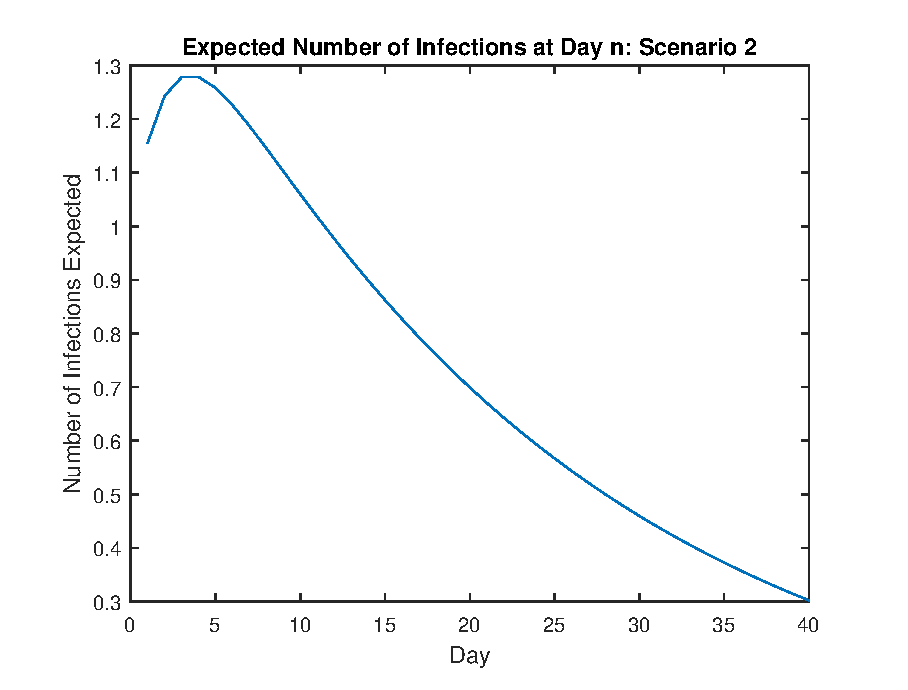
\includegraphics{expectedsc2}
\end{figure}
\begin{figure}[bp]
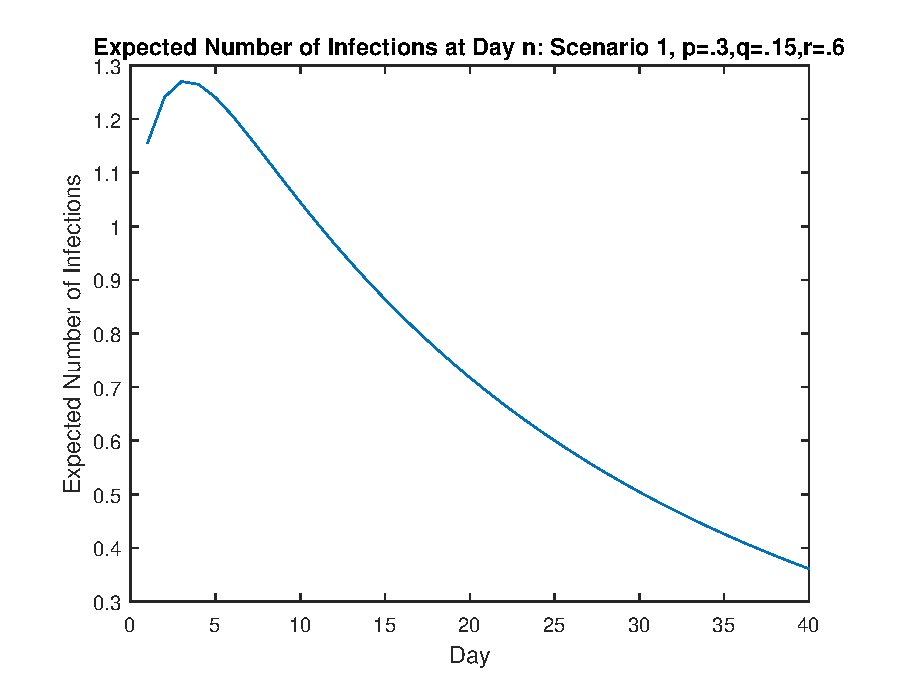
\includegraphics{expectedsc1}
\end{figure}
\pagebreak
\begin{figure}[tp]
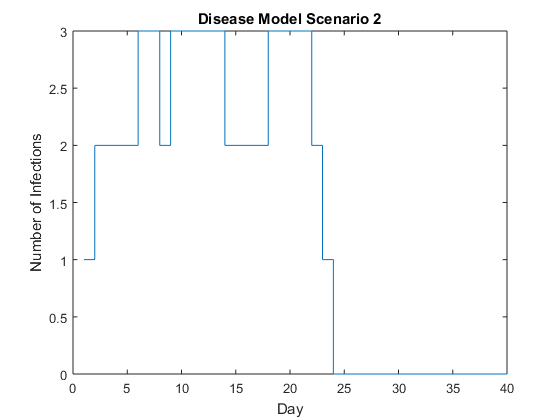
\includegraphics{modelsc2a}
\end{figure}
\begin{figure}[bp]
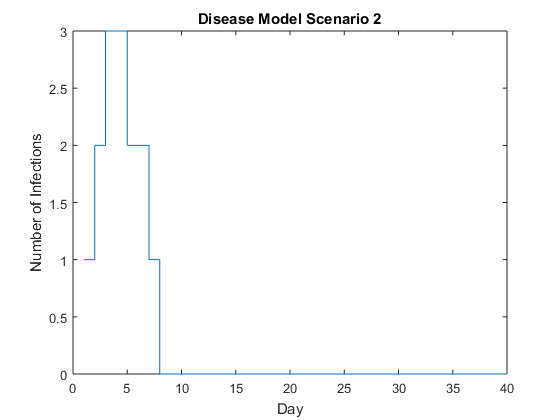
\includegraphics{modelsc2b}
\end{figure}
\begin{figure}[tp]
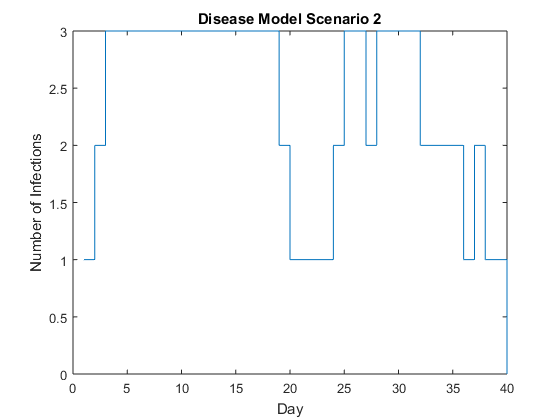
\includegraphics{modelsc2c}
\end{figure}
\begin{figure}[bp]
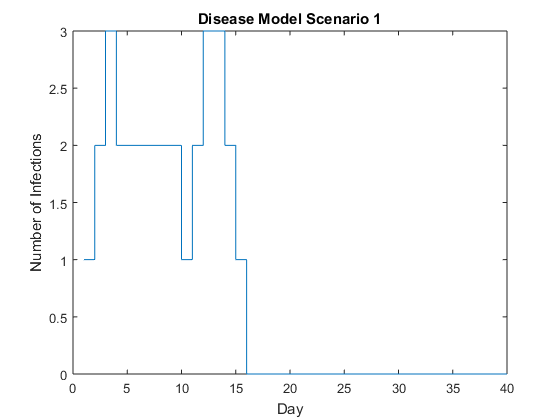
\includegraphics{modelsc1a}
\end{figure}
\begin{figure}[tp]
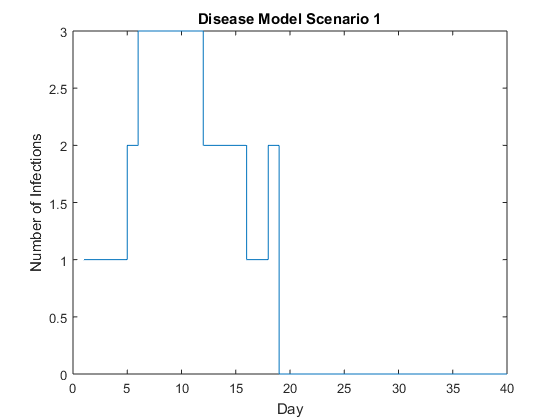
\includegraphics{modelsc1b}
\end{figure}
\begin{figure}[bp]
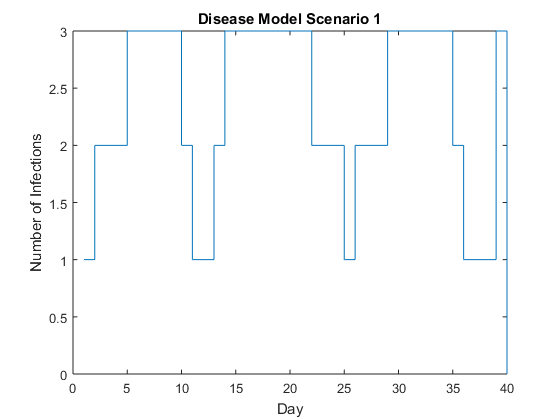
\includegraphics{modelsc1c}
\end{figure}
\begin{figure}[tp]
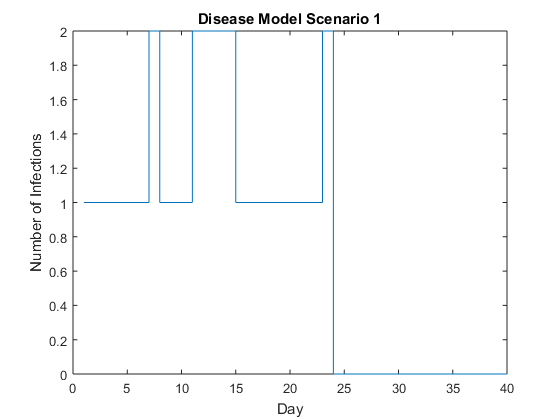
\includegraphics{modelsc1d}
\end{figure}
\end{document}